\documentclass[a4paper,10pt]{scrartcl}
\usepackage[utf8]{inputenc}
\usepackage[T1]{fontenc}
\usepackage{booktabs}
\usepackage{import}
\usepackage{xspace}
\usepackage{enumitem}
\usepackage{cite}
\usepackage{graphicx}
\usepackage{tikz}
\usetikzlibrary{arrows}
\usetikzlibrary{fit}
\usetikzlibrary{calc}
\usepackage{float}
\usepackage{amssymb}
\usepackage{listings}
\usepackage[section]{placeins} % don't move figures beyond the next section heading

% this is needed for forms and links within the text
\usepackage{hyperref}

% Variables
\newcommand{\authorName}{
   Mohammed~Abu~Jayyab,
   Niklas~Baumstark,
   Tobias~Gräf,
   Amrei~Loose,
   Christoph~Michel,
}
\newcommand{\authorNameEmph}{
   Mohammed~Abu~Jayyab,
   Niklas~Baumstark,
   \textbf{Tobias~Gräf},
   Christoph~Michel,
   Amrei~Loose,
}

\newcommand{\dateFirstVersion}{\today}
\newcommand{\customer}{Karlsruhe Institute of Technology}
\newcommand{\contractor}{A company}
\newcommand{\projectName}{Broadcast Encryption\xspace}

\newcommand{\doctitle}{\projectName (Design document)}
\title{\doctitle}
\author{\authorName}
\date{\today}

% less margin
\usepackage[margin=2.5cm]{geometry}

% horizontal line
\newcommand{\HRule}{\rule{\linewidth}{0.5mm}}

% more beautiful lists
\setlist{noitemsep}
\renewcommand{\labelitemi}{$\bullet$}
\renewcommand{\labelitemii}{$\diamond$}

% create a shorter version for tables
\newcommand\addrow[2]{#1 &#2\\ }
\newcommand\addheading[2]{\textbf{\sffamily #1} &\textbf{\sffamily #2}\\ \hline}
\newcommand\tabularhead{\begin{tabular}{lp{13cm}}
\hline
}

\newcommand\addmulrow[2]{ \begin{minipage}[t][][t]{2.5cm}#1\end{minipage}%
   &\begin{minipage}[t][][t]{8cm}
    \begin{enumerate} #2   \end{enumerate}
    \end{minipage}\\ }

\newenvironment{usecase}{\tabularhead}
{\hline\end{tabular}}

% a cross
\newcommand\X{$\times$}

% templates and default styles for figures and graphics
\tikzset{>=triangle 45}
\tikzset{font=\sffamily}

\newcommand{\tmpCaption}{}
\newenvironment{illustration}[1]
{
   \renewcommand{\tmpCaption}{#1}
   \begin{figure}[h!]
   \centering
}
{
   \caption{\tmpCaption}
   \end{figure}
}


\begin{document}

\maketitle
  \begin{tabular}[t]{ll}
	Projekt:       & \quad \projektName \\[1.2ex]
	Auftraggeber:  & \quad \auftraggeber\\[1.2ex]
	Auftragnehmer: & \quad \auftragnehmer\\[1.2ex]
  \end{tabular}

\begin{tabular}{|p{3 cm}|p{3 cm}|p{5 cm}|}
\hline
\textbf{Version} & \textbf{Datum} & \textbf{Autor(en)} \\
\hline
\hline
1.0 & 29.04.2012 & \authorName \\
\hline
\end{tabular}

\tableofcontents
\clearpage

\section{Introduction}
%CryptoCast is a piece of software that provides a service to send contents from a central server to a given
%group of recipients. Transmission happens via a unidirectional communication channel like IP multicast.
%The traffic duplication that would be required for commonly used transport protocols is therefore avoided.

%It enables access control through a specific form of encryption that is based on the Naor-Pinkas broadcast
%encryption scheme. The advantage of this scheme is the 

The software CryptoCast will provide a service for sending encrypted data from a server to certain
amount of people.  This will be implemented as an unidirectional connection that makes it possible for the server
to send data without knowing how many people are receiving it and without the amount of traffic caused
by a bidirectional connection.  Also the type of the sent data will not be determined by the software. So it can be
used for all sorts of data exchange. For demonstration purposes we will implement a simple audio or video stream.

The server will be able to register new users and revoke specific persons if they are not allowed to receive the cast anymore. 
The client is an app on an Android smart phone that is used for receiving, decoding and displaying the data. 
The transport between them will be implemented with TCP but that can be replaced by another transport protocoll.

The implemented encryption algorithm will be the one by Moni Naor and Benny Pinkas, but later every other fitting the
interface can be used. This is important because there might be another more effective algorithm that can replace the implemented one.

In our design we will therefore focuse on modularity and encapsulation to enable substitution for parts of the programm without having to 
change a lot of their enviroment.

\section{Structure}
\subsection{Architecture}
The server will be designed with a three tier architecture, containing layers for presentation, application and data. In our case 
the presentation layer is presented by the shell, the application layer consists of the controller and the data layer contains ServerData and Command. Dividing the server into those layers makes the different parts less complex and it is possible to modify one layer without having to change the others.

\begin{illustration}{3-tier architecture of the server}

\tikzset{
  rect/.style={draw,fill=green!15,minimum height=0.8cm,rectangle},
  box/.style={
    draw=blue!50!white,
    line width=1pt,
    dash pattern=on 1pt off 4pt on 6pt off 4pt,
    inner sep=4mm, rectangle, rounded corners
  },
}

\begin{tikzpicture}[auto,node distance=1.5cm]

\node[rect,minimum width=6cm](shell) {\textbf{Shell}};
\node[rect,minimum width=3cm,xshift=-1.5cm,below of=shell](control) {Controller};;
\node[rect,minimum width=3cm,below of=control](data) {ServerData};
\node[rect,minimum width=2cm,xshift=2cm, right of=data](cmd) {Command};

\draw [<->]  (shell.south) --  (control.north)
;
\draw [->]  (shell.south) --  (cmd.north)
  ;
\draw [->]  (control.south) --  (data.north)
  ;

\end{tikzpicture}

\end{illustration}

\section{Package descriptions}
\subimport{../docs/}{all.tex}

\section{Sequences}
\begin{illustration}{Sequence diagram of a command perfomed by the Server.}
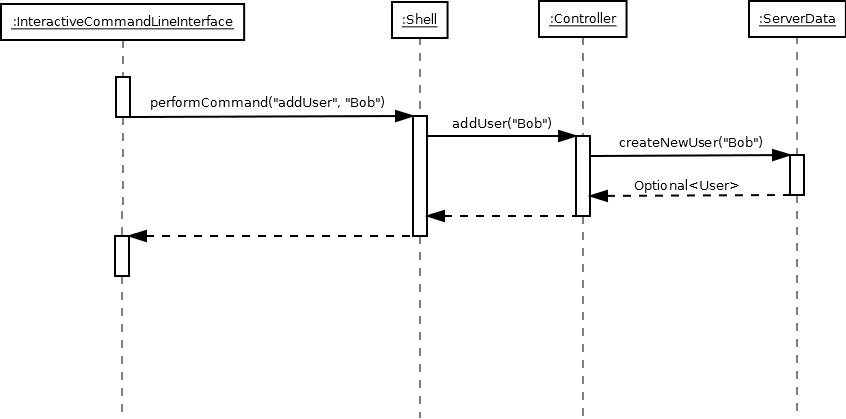
\includegraphics [width=400px] {figures/sequence_diagramm_server/Server1.png}
\end{illustration}
\begin{illustration}{Sequence diagram of playing a stream for the first time.}
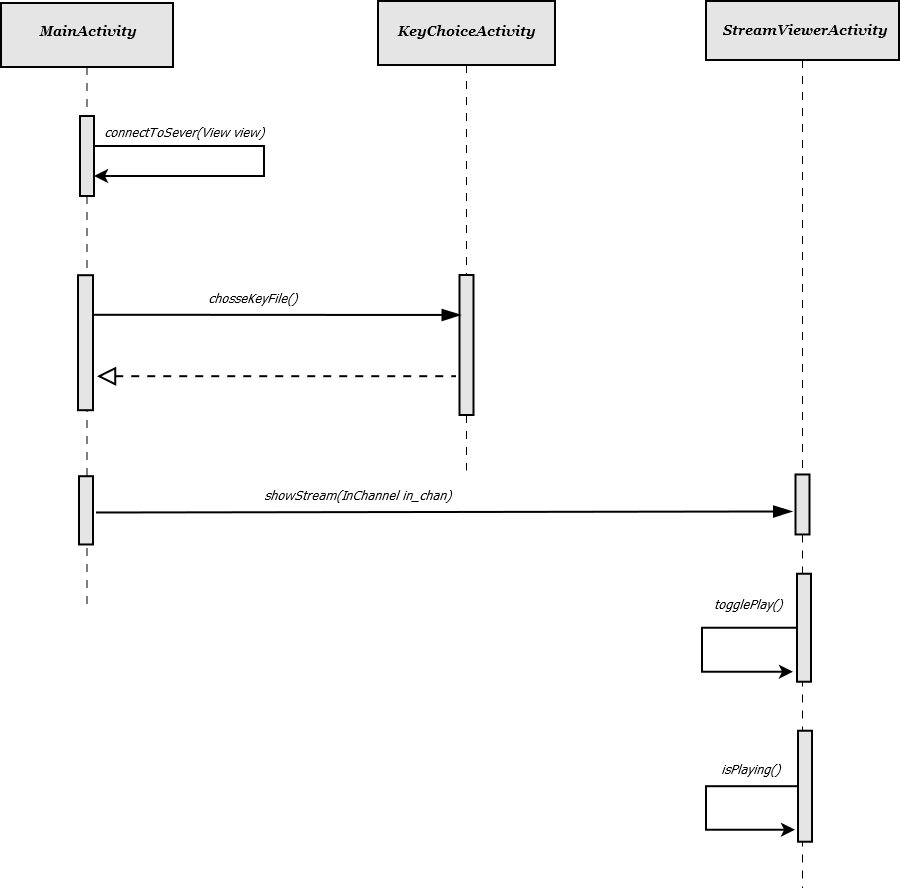
\includegraphics [width=400px] {figures/sequence_digram_client/sequence_client.png}
\end{illustration}



%\bibliography{../bibtex/references}{}
%\bibliographystyle{plain}

\section{GUI design}
The GUI should be user-friendly and intuitional. Therefore its design is very minimalistic, foccusing on its main purpose. 
The following images show prototypes of the graphical user interface.

\begin{illustration}{The main screen which is shown on program start. (The empty space is used for the logo later on))}
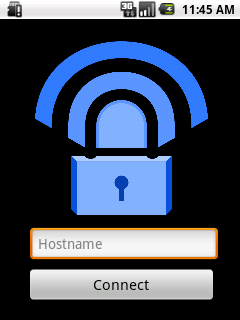
\includegraphics[width=150px]{figures/images/mainscreen.png}
\end{illustration}
\begin{illustration}{The menu which pops up after the menu button is pressed. It allows navigation between the different screens.}
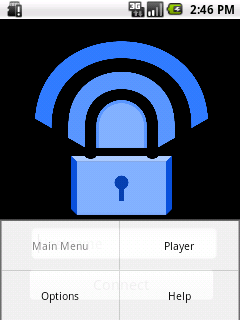
\includegraphics[width=150px]{figures/images/menu.png}
\end{illustration}
\begin{illustration}{The option screen which contains preferences, traffic data and a server history.}
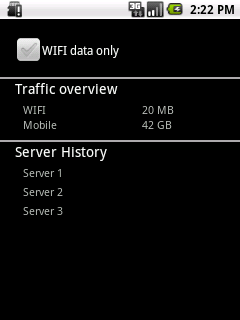
\includegraphics[width=150px]{figures/images/optionscreen.png}
\end{illustration}

\end{document}
